\section{METODOLOGIA}

O trabalho desenvolvido consiste em uma pesquisa aplicada na relação da ética no desenvolvimento em robótica. Assim ela parte de uma abordagem qualitativa do problema, sendo ele analisado a partir de diversas óticas.

Dessa maneira foi feita uma revisão bibliográfica de artigos relacionados ao tema central da pesquisa. A pesquisa foi feita utilizando o \textit{método bili} \cite{Brazilia89:online} para partir de um objetivo geral para um objetivo específicos e encontrar os artigos mais relevantes ao tema.  

\begin{figure}[h!]
   \centering
       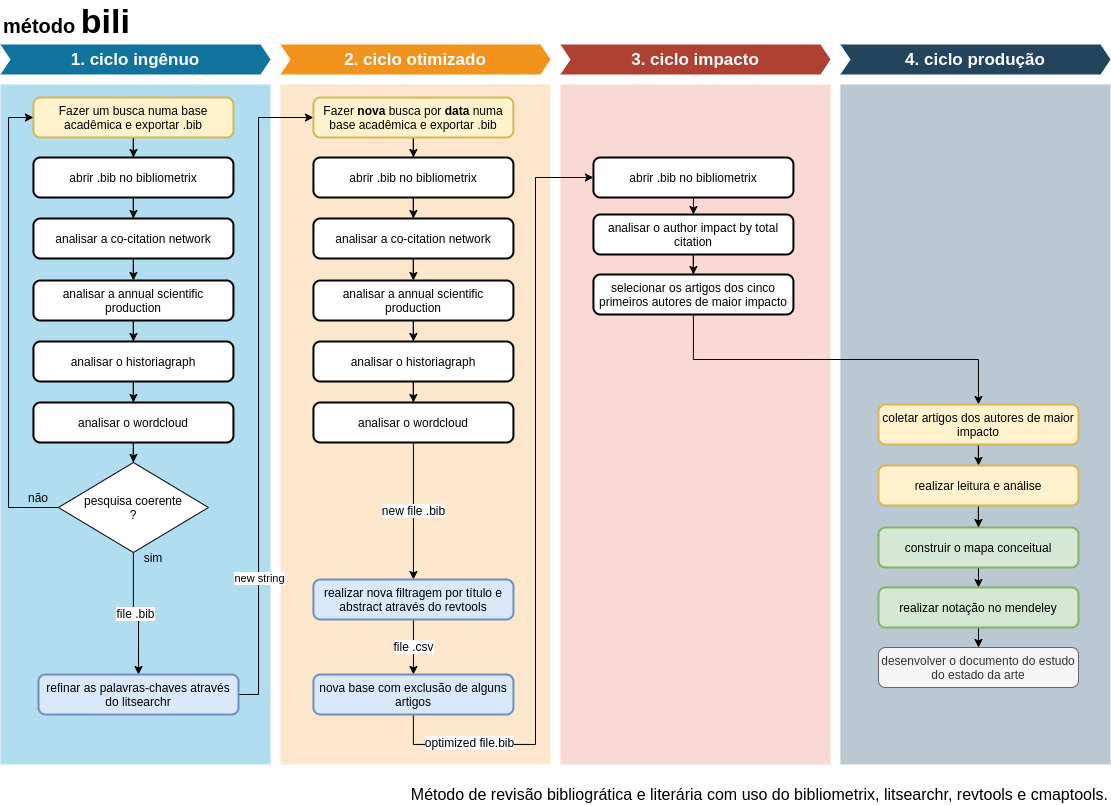
\includegraphics[width=15cm]{source/pictures/bili.png}
   \caption{***Colocar   citação}
   \label{fig:bili}
\end{figure}

Como mostrado na figura \ref{fig:bili} o método de pesquisa utilizado é composto por quatro ciclo: ingênuo, otimizado, impacto e produção. Essas fazes consistem em fazer analises estatísticas para se definir um foco de pesquisa, analisar sua relevância e encontrar artigos mais importantes. Assim essas partes serão melhor detalhadas

\subsection{Ciclo ingênuo}
Utilizando-se do site do \textit{Scopus} foram realizadas buscas através de palavras chaves relacionadas ao tema de etica na robotica. Com isso coletou-se os nartigos e gerou-se um arquivo do tipo \textit{bibtex}. Esse arquivo foi colocado em uma ferramenta denominada \textit{Bibliometrix}. Nessa ferramenta foi feito a analise desse arquivo.

Com o \textit{Bibliometrix} foi analisado, primeiramente, o \textit{anual scientific production}, mostra a quantidade de artigos publicados por ano. Em seguida, foi analisado o \textit{co-citation network}, onde se verifica se os artigos estão relacionados entre si. Após isso foram analisados o \textit{historiograph} e o \textit{wordcloud}.

Essa etapa do projeto foi repetida algumas vezes até que se encontraram-se resultados coerentes. Com esses resultados foi utilizado i \textit{litsearch} para refinar ainda mais os resultados.

\subsection{Ciclo otimizado}

Com o novo resultado do ciclo anterior foi feito uma nova analise dos resultados obtidos. A partir dai foram feitas as leituras do titulo e do abstract dos artigos restantes para retirar os artigos que não esteja, relacionados ao tema da pesquisa. Gerando assim um novo arquivo a ser analisado.

\subsection{Ciclo impacto}

Esse novo arquivo é aberto novamente no \textit{Bibliometrix}, onde os autores de maior impacto são selecionados. Com isso seus artigo são selecionados e lidos na proxima etapa.

\subsection{Ciclo produção}

Nessa etapa é onde os artigo de maior impacto são estudados. Produzindo assim mapas conceituais e anotações de cada artigo. Assim é gerado um documento de estudo do estado da arte e o artigo começa a ser escrito.